Gegeben ist die Matrix
\[
A
=
\begin{pmatrix}
 1 & 3 & 8 \\
 8 & 2 & 2
\end{pmatrix}.
\]
\begin{teilaufgaben}
\item Berechnen Sie die symmetrischen Matrizen $B_2=AA^t$ und $B_3 = A^tA$.
\item Berechnen Sie die Eigenwerte der Matrix $B_2$.
\item Verwenden Sie den Jacobi-Rechner, um die Eigenwerte von $B_3$ zu berechnen.
\item Bestimmen Sie die Singulärwerte von $A$.
\end{teilaufgaben}
\begin{hinweis}
\vspace*{-0.6cm}
QR-Codes für Jacobi-Rechner: $AA^t=$
\hspace*{-0.3cm}
\raisebox{-1.10cm}{%
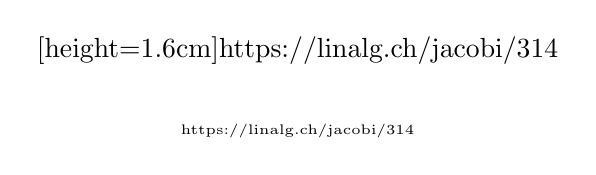
\begin{tikzpicture}[>=latex,thick]
\node at (0,0) {\qrcode[height=1.6cm]{https://linalg.ch/jacobi/314}};
\node at (0,-0.8) [below] {\tiny https://linalg.ch/jacobi/314};
\end{tikzpicture}}
\hspace*{-0.3cm},
\;
$A^tA=$
\raisebox{-1.10cm}{%
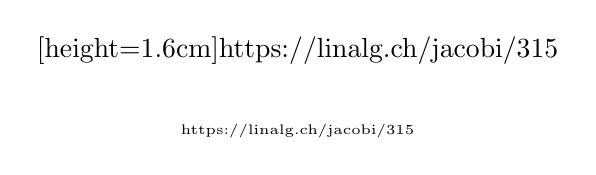
\begin{tikzpicture}[>=latex,thick]
\node at (0,0) {\qrcode[height=1.6cm]{https://linalg.ch/jacobi/315}};
\node at (0,-0.8) [below] {\tiny https://linalg.ch/jacobi/315};
\end{tikzpicture}}
\hspace*{-0.2cm}.
\end{hinweis}

\begin{loesung}
\begin{teilaufgaben}
\item
Die beiden Matrizen sind
\begin{align*}
B_2
&=
AA^t
=
\begin{pmatrix}
 1 & 3 & 8 \\
 8 & 2 & 2
\end{pmatrix}
\raisebox{-0.22cm}{$\displaystyle
\begin{pmatrix}
 1 & 8 \\
 3 & 2 \\
 8 & 2
\end{pmatrix}$}
=
\begin{pmatrix}
74&30\\
30&72
\end{pmatrix}
\\
B_3
&=
A^tA
=
\begin{pmatrix}
 1 & 8 \\
 3 & 2 \\
 8 & 2
\end{pmatrix}
\raisebox{0.22cm}{$\displaystyle
\begin{pmatrix}
 1 & 3 & 8 \\
 8 & 2 & 2
\end{pmatrix}$}
=
\begin{pmatrix}
   65 & 19 & 24 \\
   19 & 13 & 28 \\
   24 & 28 & 68
\end{pmatrix}.
\end{align*}
\item
Die Eigenwerte von $B_2$ sind die Nullstellen des charakteristischen Polynoms
\begin{align*}
\det(B_2-\lambda I)
=
\left|
\begin{matrix}
74 - \lambda &     30      \\
     30     & 72 - \lambda
\end{matrix}
\right|
&=
(74-\lambda)(72-\lambda) - 900
\\
&=
74\cdot 72 - 146\lambda + \lambda^2 -900
\\
&=
\lambda^2-146\lambda+4428.
\end{align*}
Die Lösungsformel für die quadratische Gleichung liefert
\begin{align*}
\lambda_{\pm}
&=
73\pm\sqrt{73^2-4428}
=
73\pm\sqrt{901}
=
\begin{cases}
103.017\\
\phantom{0}42.983.
\end{cases}
\end{align*}
\item $B_3$ hat Rang 2 und daher einen Eigenwert 0, die anderen zwei Eigenwerte stimmen
mit den Eigenwerten von $B_2$ überein.
\item
Die Singulärwerte sind die Wurzeln der Nullstellen $\lambda_\pm$, also
\begin{align*}
\sigma_1
&=
\sqrt{\lambda_+}
=
10.1497
\\
\sigma_2
&=
\sqrt{\lambda_-}
=
\phantom{0}
6.5562
\qedhere
\end{align*}
\end{teilaufgaben}
\end{loesung}

